Fitting the anomalous couplings one at a time while fixing the other couplings
to the Standard Model values, we get the following results:

%%  **********
%%  **   24 **MINOS        3000
%%  **********
%%  MINUIT WARNING IN HESSE
%%  FCN=34.6312 FROM MINOS     STATUS=PROBLEMS      431 CALLS         737 TOTAL
%%                      EDM=1.7308e-09    STRATEGY= 1  ERROR MATRIX UNCERTAINTY 100.0 per cent
%%   EXT PARAMETER                  PARABOLIC         MINOS ERRORS        
%%   NO.   NAME      VALUE            ERROR      NEGATIVE      POSITIVE   
%%    1  n_top        5.33068e+01   9.75132e+02   at limit      at limit   
%%    2  n_wjets      9.53674e-04   8.44316e+02   at limit      at limit   
%%    3  n_ww         1.13063e+01   2.54938e+00  -2.51146e+00   2.57877e+00
%%    4  n_wz         9.53674e-04   8.44316e+02   at limit      at limit   
%%    5  n_zz         6.07414e+01   6.92371e+02   at limit      at limit   
%%    6  x_par       -3.24099e-04   1.86003e-01  -1.88409e-01   1.89906e-01
%%                                ERR DEF= 1.92

%%  **********
%%  **   24 **MINOS        3000
%%  **********
%%  MINUIT WARNING IN HESSE
%%  FCN=34.629 FROM MINOS     STATUS=PROBLEMS      450 CALLS         756 TOTAL
%%                      EDM=1.16249e-11    STRATEGY= 1  ERROR MATRIX UNCERTAINTY 100.0 per cent
%%   EXT PARAMETER                  PARABOLIC         MINOS ERRORS        
%%   NO.   NAME      VALUE            ERROR      NEGATIVE      POSITIVE   
%%    1  n_top        5.33068e+01   5.44898e+02   at limit      at limit   
%%    2  n_wjets      9.53674e-04   8.44316e+02   at limit      at limit   
%%    3  n_ww         1.13063e+01   2.54938e+00  -2.51142e+00   2.57866e+00
%%    4  n_wz         9.53674e-04   8.44316e+02   at limit      at limit   
%%    5  n_zz         6.07414e+01   6.92371e+02   at limit      at limit   
%%    6  y_par        9.91721e-03   2.91058e-01  -3.00825e-01   3.02058e-01
%%                                ERR DEF= 1.92

%%  **********
%%  **   24 **MINOS        3000
%%  **********
%%  MINUIT WARNING IN HESSE
%%  FCN=34.279 FROM MINOS     STATUS=PROBLEMS      450 CALLS         497 TOTAL
%%                      EDM=4.34025e-09    STRATEGY= 1  ERROR MATRIX UNCERTAINTY 100.0 per cent
%%   EXT PARAMETER                  PARABOLIC         MINOS ERRORS        
%%   NO.   NAME      VALUE            ERROR      NEGATIVE      POSITIVE   
%%    1  n_top        6.07414e+01   8.76615e+02   at limit      at limit   
%%    2  n_wjets      9.53674e-04   8.44316e+02   at limit      at limit   
%%    3  n_ww         1.13063e+01   2.54938e+00  -2.51134e+00   2.57871e+00
%%    4  n_wz         9.53674e-04   8.44316e+02   at limit      at limit   
%%    5  n_zz         6.07414e+01   6.92371e+02   at limit      at limit   
%%    6  y_par        1.86593e-02   5.97146e-01  -6.32675e-01   6.34256e-01
%%                                ERR DEF= 1.92

\fixme{Update results}

\begin{align}
  \lambda_{Z} &= 0.00\pm0.19, ~95\%~\mathrm{C.L.} \\ 
  \Delta g^Z_1 &= 0.01\pm0.30, ~95\%~\mathrm{C.L.}\\
  \Delta\kappa_\gamma &= 0.02\pm0.63, ~95\%~\mathrm{C.L.}\\
\end{align}

\fixme{What do we do with coverage? Ignore for now}

Sampling \wwll\ Monte Carlo events we find that within the reported 95\%
confidence limits $\lambda_{Z}$ contained $97\pm1$\% and
$\Delta\kappa_{Z}$ contained $94\pm1$\% of the test samples.

\fixme{Update numbers}
Most systematic uncertainties were included in the fit as Gaussian
constraints. The following constraints were used:
\begin{itemize}
  \item expected Standard Model \ww\ event yield: $10.8\pm1.4$ ( 11\%
    (lumi) $\oplus$ 7\% (eff) $\oplus$ 5\%($\sigma_{\ww}$) )
  \item top background: $0.85\pm0.85$
  \item \wjets\ and Drell-Yan: $2.1\pm0.7$
  \item \wz{}: $0.2\pm0.2$
  \item \zz{}: $0.10\pm0.01$
\end{itemize}

\fixme{Update}

Final exclusion limits for anomalous couplings are:
\begin{align}
  \lambda_{Z}: [-0.19,0.19]~95\%~\mathrm{C.L.}\\ 
  \Delta\kappa_{Z}: [-0.29,0.31]~95\%~\mathrm{C.L.}\\
  \Delta\kappa_\gamma: [-0.61,0.65]~95\%~\mathrm{C.L.}\\
\end{align}

Figure~\ref{fig:contourL} and Figure~\ref{fig:contour} show 2D
confidence limit contour plots for anomalous
couplings. Figure~\ref{ref:likelihood} shows a likelihood scan.

\begin{figure}[tp]
  \centerline{
    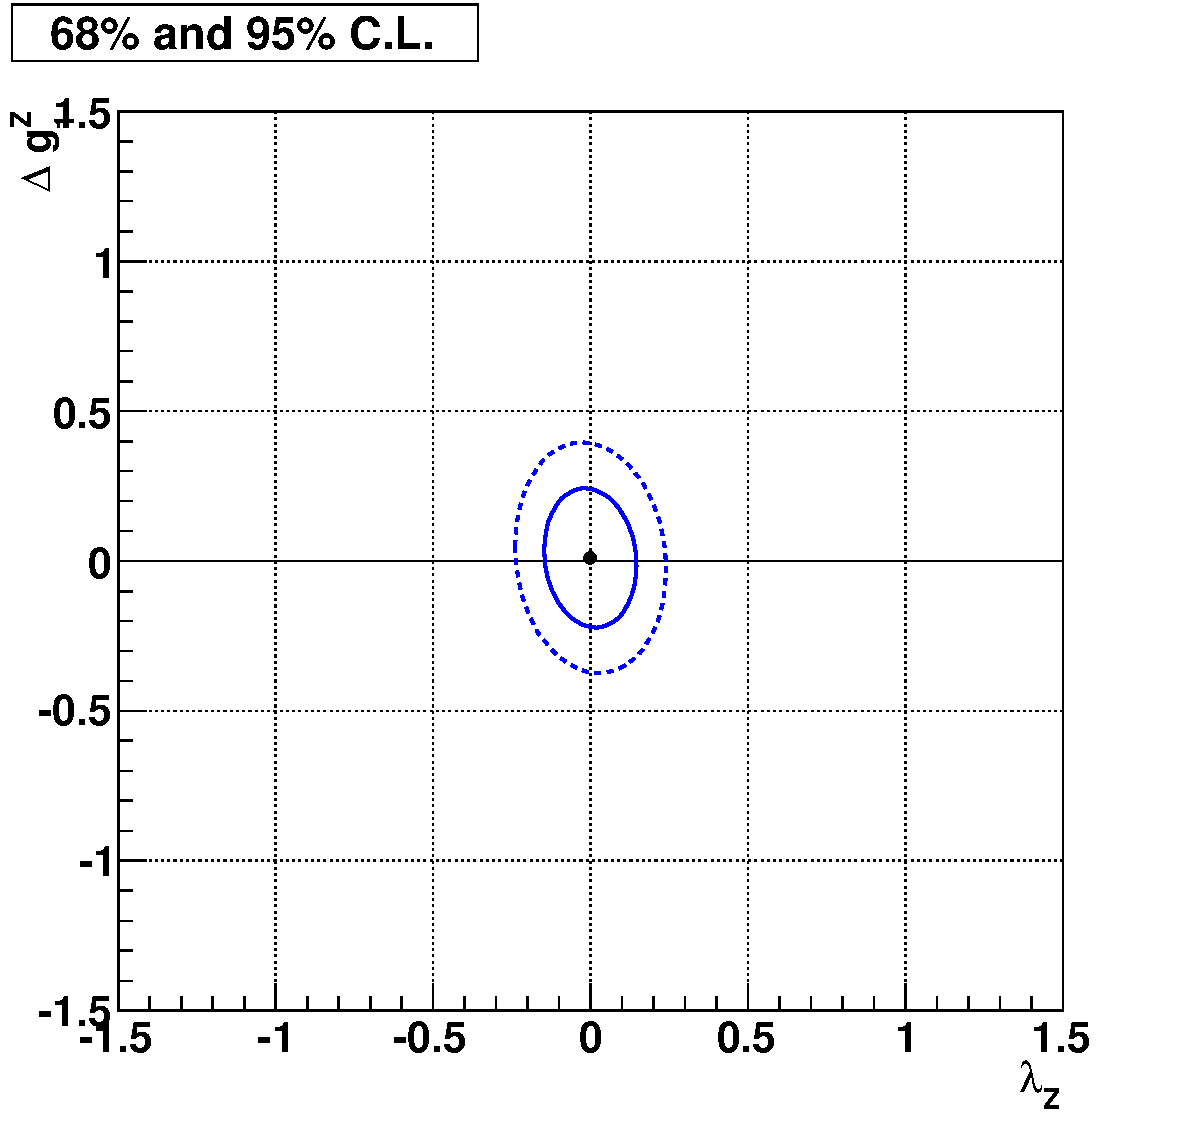
\includegraphics[width=0.5\textwidth]{figures/lz_dkz_contourplot2}
    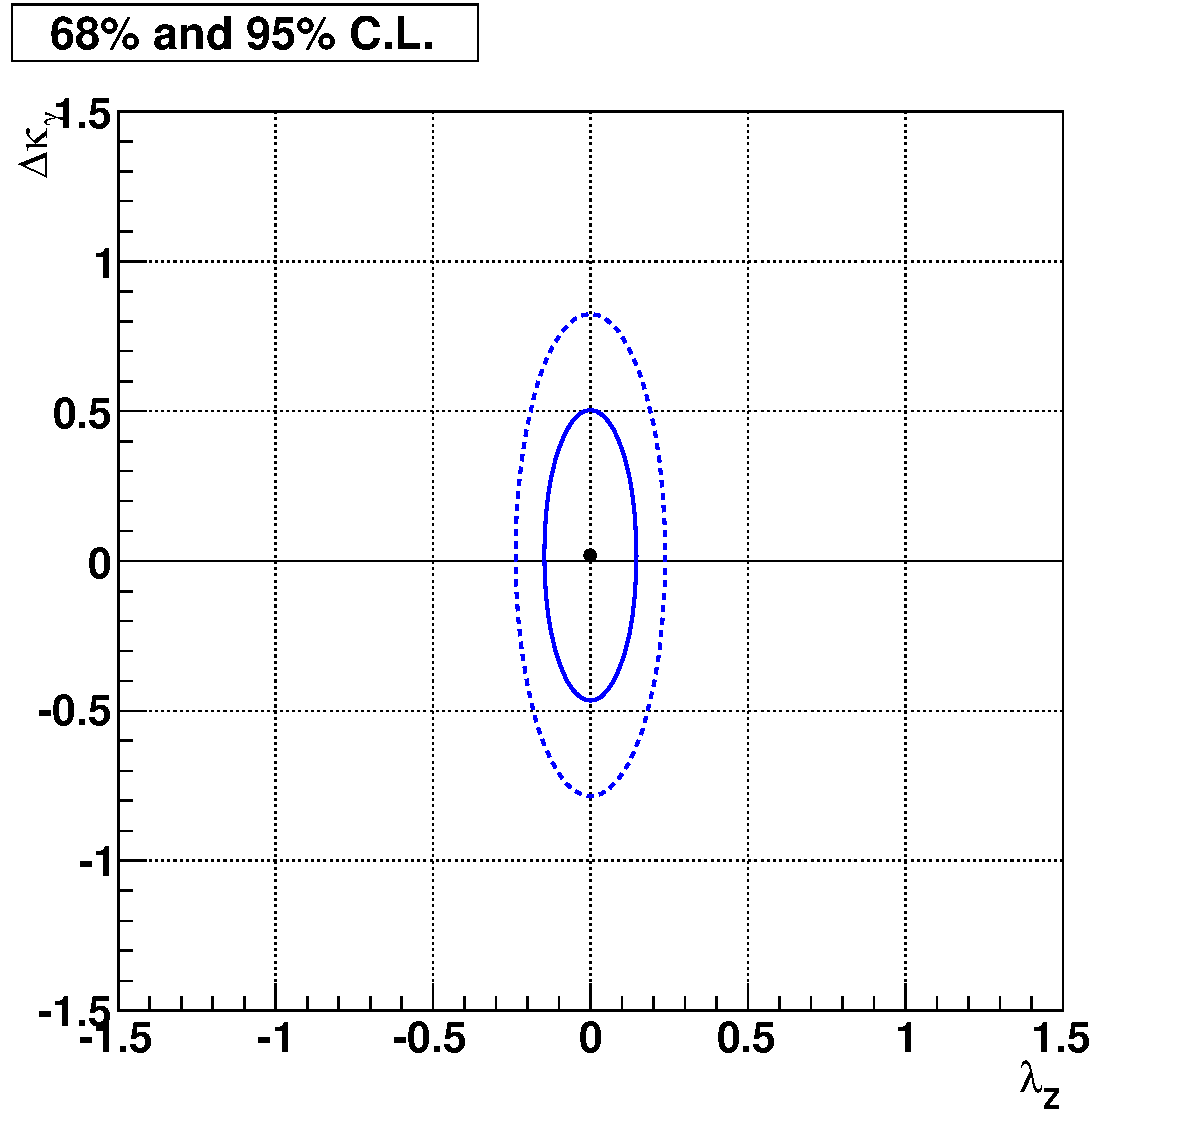
\includegraphics[width=0.5\textwidth]{figures/lz_dkg_contourplot2}
  }

  \caption[Contour plots for data] {aTGC 68\% and 95\% C.L. contour
    plots for a model without form factors for 35.5\ipb\ of data.}
  \label{fig:contour}
\end{figure}

\begin{figure}[tp]
  \centerline{
    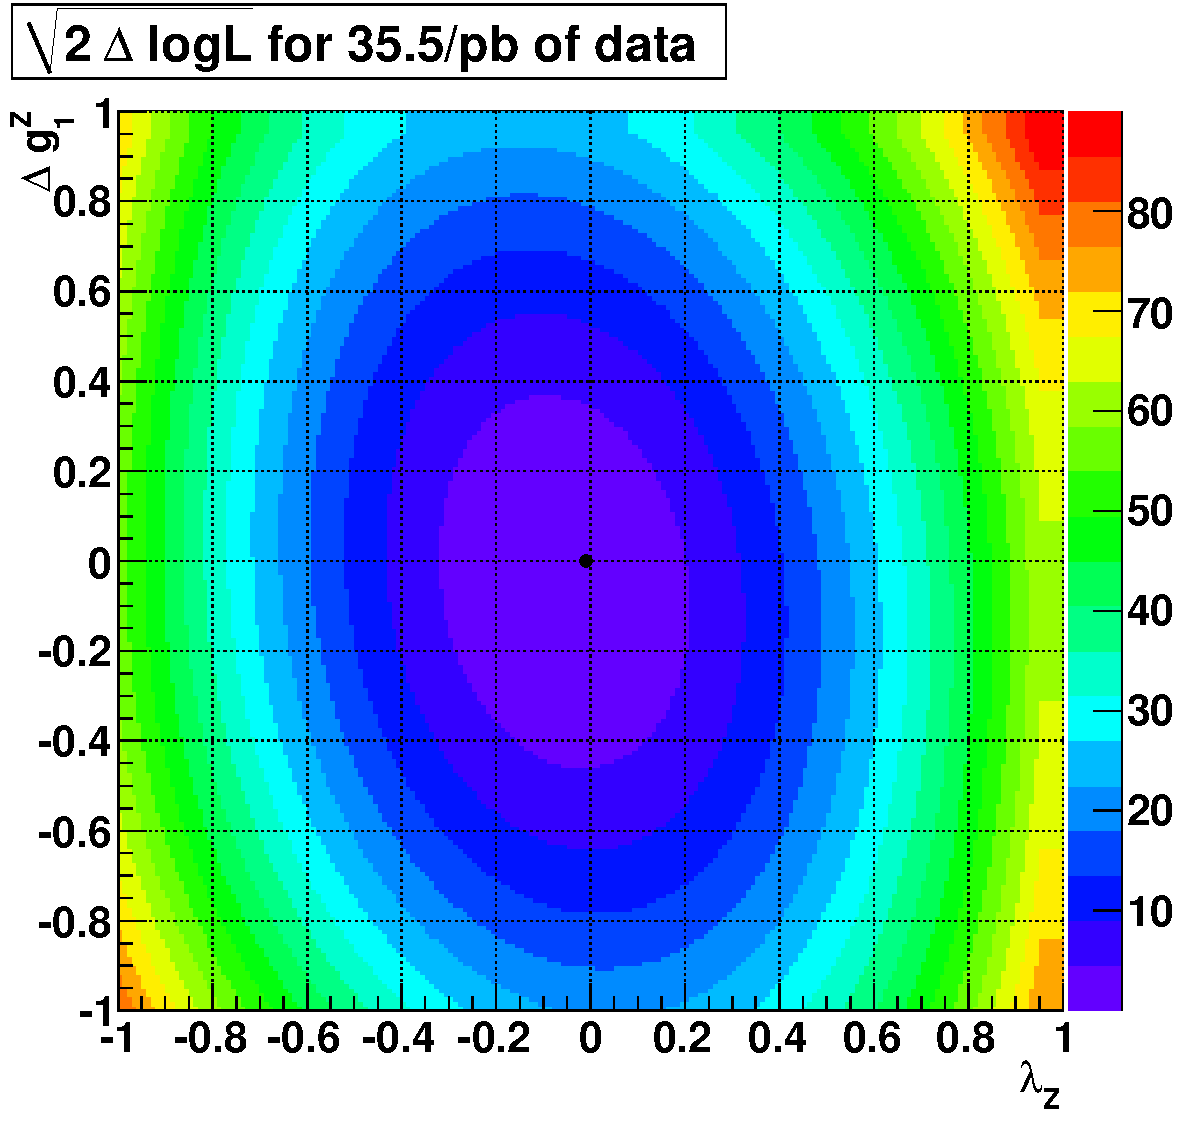
\includegraphics[width=0.5\textwidth]{figures/lz_dkz_likelihood.pdf}
  }

  \caption[Likelihood scan] {Likelihood scan ($\sqrt{2\Delta\log L}$)
    for XXX\ipb\ of  data. }
  \label{ref:likelihood}
\end{figure}
